% !TEX encoding = UTF-8 Unicode
\documentclass[a4paper]{article}

\usepackage{color}
\usepackage{url}
\usepackage[utf8]{inputenc} % make weird characters work

\usepackage{graphicx}
\graphicspath{ {./images/} }


\usepackage[english,serbian]{babel}
\usepackage{booktabs} % To thicken table lines
\usepackage{adjustbox}
\usepackage[bottom]{footmisc}
\usepackage{amsfonts}
\usepackage{amsmath}


\usepackage[]{algorithm2e}
\usepackage{subcaption}

\usepackage[margin=1cm]{caption}

\usepackage{tabularx}  % for 'tabularx' environment and 'X' column type
\usepackage{ragged2e}  % for '\RaggedRight' macro (allows hyphenation)
\newcolumntype{Y}{>{\RaggedRight\arraybackslash}X} 


\usepackage{float} % here for H placement parameter
\usepackage[a4paper,left=3cm,right=3cm,top=3cm,bottom=3cm]{geometry}




\usepackage{tikz}
\usetikzlibrary{decorations.pathreplacing}
\newcommand{\tikzmark}[1]{\tikz[overlay,remember picture] \node[baseline] (#1) {};}
\tikzset{My Node Style/.style={midway, right, xshift=3.0ex, align=left, font=\small, draw=none, thin, text=black}}



\usepackage[unicode]{hyperref}
\hypersetup{colorlinks,citecolor=green,filecolor=green,linkcolor=blue,urlcolor=blue}

\usepackage{listings}

%\newtheorem{primer}{Primer}[section]

\definecolor{mygreen}{rgb}{0,0.6,0}
\definecolor{mygray}{rgb}{0.5,0.5,0.5}
\definecolor{mymauve}{rgb}{0.58,0,0.82}

\lstset{ 
  backgroundcolor=\color{white},   % choose the background color; you must add \usepackage{color} or \usepackage{xcolor}; should come as last argument
  basicstyle=\scriptsize\ttfamily,        % the size of the fonts that are used for the code
  breakatwhitespace=false,         % sets if automatic breaks should only happen at whitespace
  breaklines=true,                 % sets automatic line breaking
  captionpos=b,                    % sets the caption-position to bottom
  commentstyle=\color{mygreen},    % comment style
  deletekeywords={...},            % if you want to delete keywords from the given language
  escapeinside={\%*}{*)},          % if you want to add LaTeX within your code
  extendedchars=true,              % lets you use non-ASCII characters; for 8-bits encodings only, does not work with UTF-8
  firstnumber=1000,                % start line enumeration with line 1000
  frame=single,	                   % adds a frame around the code
  keepspaces=true,                 % keeps spaces in text, useful for keeping indentation of code (possibly needs columns=flexible)
  keywordstyle=\color{blue},       % keyword style
  language=Python,                 % the language of the code
  morekeywords={*,...},            % if you want to add more keywords to the set
  numbers=left,                    % where to put the line-numbers; possible values are (none, left, right)
  numbersep=5pt,                   % how far the line-numbers are from the code
  numberstyle=\tiny\color{mygray}, % the style that is used for the line-numbers
  rulecolor=\color{black},         % if not set, the frame-color may be changed on line-breaks within not-black text (e.g. comments (green here))
  showspaces=false,                % show spaces everywhere adding particular underscores; it overrides 'showstringspaces'
  showstringspaces=false,          % underline spaces within strings only
  showtabs=false,                  % show tabs within strings adding particular underscores
  stepnumber=2,                    % the step between two line-numbers. If it's 1, each line will be numbered
  stringstyle=\color{mymauve},     % string literal style
  tabsize=2,	                   % sets default tabsize to 2 spaces
  title=\lstname                   % show the filename of files included with \lstinputlisting; also try caption instead of title
}

%\usepackage{apacite}















\begin{document}

\title{Klasterovanje PBMC uzoraka\\\small{Seminarski rad u okviru kursa\\Istraživanje podataka 2\\ Matematički fakultet}}

\author{
  Košanin Petar\\
  \texttt{mi15140@matf.bg.ac.rs}
    \and
  Gružanić Nemanja\\
  \texttt{mi16420@matf.bg.ac.rs}
}

\maketitle


\abstract{PBMC (eng. Peripheral Blood Mononuclear Cells) su krvne ćelije kod kojih je prisutan jedan ovalni nukleus. PBMC se koriste u istraživanju raznih infektivnih bolesti, imunologiji, kao i u razvoju vakcina. U ovom radu predstavićemo nekoliko algoritama klasterovanja nad podacima dobijenim kombinovanjem više različitih skupova podataka različitih istraživanja. 


\smallskip
\noindent \textit{\textbf{Ključne reči:}} \textit{PBMC}, \textit{klasterovanje} \textit{spektralno klasterovanje}, \textit{nenegativna faktorizacija}

}


\tableofcontents

\newpage







\section{Uvod}
PBMC (eng. Peripheral Blood Mononuclear Cells) su krvne ćelije kod kojih je prisutan jedan ovalni nukleus. PBMC se koriste u istraživanju raznih infektivnih bolesti, imunologiji, kao i u razvoju vakcina. Podaci su sakupljeni iz više različitih izvora \cite{shaikh2019classification}. U nastavku biće reči o njihovoj inicijalnoj formi, načinu kako smo ih preprocesuirali, i konačno dobijeni rezultati klasterovanja.

\section{Podaci}

Skup podataka čini 11 datoteka i dve konsultacione datoteke. Podaci su podeljeni u dve grupe, pri čemu prvu grupu čine datoteke čiji nazivi počinju prefiksom GSM2, dok je prefiks druge grupe GSM3.

\newcommand\VerticalBrace[4][]{%
    % #1 = draw options
    % #2 = top mark
    % #2 = bottom mark
    % #4 = label
\begin{tikzpicture}[overlay,remember picture]
  \draw[decorate,decoration={brace, amplitude=1.5ex}, #1] 
    ([yshift=1ex]#2.north east)  -- ([yshift=-1ex]#3.south east)
        node[My Node Style] {#4};
\end{tikzpicture}
}



\begin{enumerate}
\item GSM2560245 \tikzmark{top 1}
\item GSM2560246
\item GSM2560247
\item GSM2560248
\item GSM2560249 \tikzmark{bottom 1}
\item GSM3087619 \tikzmark{top 2}
\item GSM3169075
\item GSM3374613
\item GSM3374614
\item GSM3478792
\item GSM3892571\tikzmark{bottom 2}
\end{enumerate}

\VerticalBrace[ultra thick, blue]{top 1}{bottom 1}{Grupa 1}
\VerticalBrace[ultra thick, blue]{top 2}{bottom 2}{Grupa 2}

Konsultaciona datoteka \textbf{common\_human\_list} sadrži nazive ljudskih gena kao i njihove identifikatore. Isečak ove datoteke je prikazan u tabeli \ref{common_human}.

\begin{center}
\begin{table}[!h]
\caption{Sadržaj konsultacione datoteke common\_human\_list}
\begin{adjustbox}{width=1\textwidth}
\begin{tabular}{llllll}
\toprule
         ENSG\_ID &          hg19 &            hg37 &            hg38 & Ensembl\_GRCh38.p12\_rel94 & GSM3717979 \\
\midrule
 ENSG00000181638 &    hg19\_ZFP41 &    grch37\_ZFP41 &    grch38\_ZFP41 &                   \#ZFP41 &     \#ZFP41 \\
 ENSG00000111875 &    hg19\_ASF1A &    grch37\_ASF1A &    grch38\_ASF1A &                   \#ASF1A &     \#ASF1A \\
 ENSG00000176142 &  hg19\_TMEM39A &  grch37\_TMEM39A &  grch38\_TMEM39A &                 \#TMEM39A &   \#TMEM39A \\
 ENSG00000177186 &    hg19\_OR2M7 &    grch37\_OR2M7 &    grch38\_OR2M7 &                   \#OR2M7 &     \#OR2M7 \\
 ENSG00000135624 &     hg19\_CCT7 &     grch37\_CCT7 &     grch38\_CCT7 &                    \#CCT7 &      \#CCT7 \\
\bottomrule
\end{tabular}
\label{common_human}
\end{adjustbox}
\end{table}
\end{center}

Druga konsultaciona datoteka \textbf{SCT-10x-Metadata\_readylist\_merged-PBMC-tasks-short-Bgd.xlsx} sadrži metapodatke za datoteke koje čine skup podataka. U tabelama \ref{group1_metadata} i \ref{group2_metadata} prikazani su metapodaci redom za prvu i drugu grupu.

\section{Preprocesiranje}

Jedan od prvih problema koji se javlja je heterogenost podataka. Inicijalno, svaka datoteka za vrste ima gene, dok kolone predstavljaju ćelije. Broj gena, kao i broj ćelija, varira od datoteke do datoteke. Takođe, razlikuju se dve metode identifikacije gena. U nekim fajlovima geni su označeni njihovim ENSG-ovima(npr. ENSG00000243485), dok u drugim, označeni su njihovim nazivima(npr. RPS10). U nastavku biće opisani načini transformisanja  naziva ćelija i gena. Zatim, podaci se transponuju, i izbacuju se ćelije i geni koji nezadovoljavaju kriterijume koji će biti opisani u nastavku. Opisane metode se koriste za konstrukciju velikog skupa podataka, kao i skupove podataka za svaku grupu pojedinačno.

\subsection{Transformacija naziva gena}

Za svaku datoteku određen je njen genom. Informacije o genomima nalaze se u konsultacionoj datoteci SCT-10x-Metadata\_readylist\_merged-PBMC-tasks-short-Bgd.xlsx. Tako na primer, za GSM2560245, genom je hg19 \ref{group1_metadata}. Zatim, ažuriraju se identifikatori gena tako što se pravi novi identifikator spajanjem odgovarajućih vrednosti kolona ENSG\_ID i kolone koja odgovara genomu datoteke koja se obrađuje iz konsultacione datoteke common\_human\_list. Za datoteku GSM2560245 i gen ZFP41, ažurirani identifikator je ENSG00000181638\_ZFP41.\footnote{Za datoteke čiji genome je grch38, imena gena su uzeta iz kolone Ensembl\_GRCh38.p12\_rel94 konsultacione datoteke.} U slučaju da se gen javlja u nekoj datoteci, ali ne postoji u common\_human\_list, on biva eliminisan. 

U konsultacionoj datoteci common\_human\_list, jedino je kolona ENSG\_ID jedinstvena. To znači da postoji naziv gena kojem odgovara više različitih ENSG-ova. U ovim situacijama, izabrali smo prvi ENSG koji odgovara datom imenu gena, dok su drugi odbačeni.

\subsection{Transformacija naziva ćelija}
Nazivi ćelija se zamenjuju sa xxx\_redniBroj, gde je xxx naziv datoteke. Na primer, ako je uzorak  GSM2741551, ćelije su označene sa GSM2741551\_1,  GSM2741551\_2,  GSM2741551\_3, ...
Nakon transformisanja naziva ćelija i identifikatora gena, podaci se transponuju, ćelije postaju instance a geni atributi tako dobijenog skupa podataka.

\subsection{Spajanje datoteka}
Kako se broj gena razlikuje od datoteke do datoteke, odredili smo zajednički presek gena za sve datoteke. Upravo ti geni čine atribute velikog (eng. bulk) skupa podataka. Ćelije su se zatim iterativno dodavale na veliki skup podataka, zadržavajući vrednosti samo za zajedničke gene. Dimenzije tako dobijenog skupa podataka su $71095 \times 12805$, tj. broj ćelija je 71095 a broj zajedničkih gena je \textbf{12805}.

\subsection{Elementi van granica}
\label{elem_van_granica}
Za veliki broj gena ne postoji neka ćelija sa nenula vrednošću. Drugim rečima, postoje dosta nula kolona. Takođe, za neke gene postoji veoma mali broj ćelija kod kojih je očitana ekspresija tog gena. Slično pravilo važi i za ćelije. Zbog ovoga, eliminisali smo gene koji imaju manje od \textbf{\%1} nenula vrednosti u velikom skupu podataka. Izbačene su i ćelije koje ne zadovoljavaju bar jedan od sledeća dva uslova:
\begin{itemize}
  \item Zbir transkripata je veći od 1000
  \item Broj ne-nula gena je veći od 500
\end{itemize}

Tako na primeru grupe 1, primenom ovih pravila, dobijamo skup podataka dimenzija $15165 \times 7545$.

%\begin{figure}[H]
%\centering
%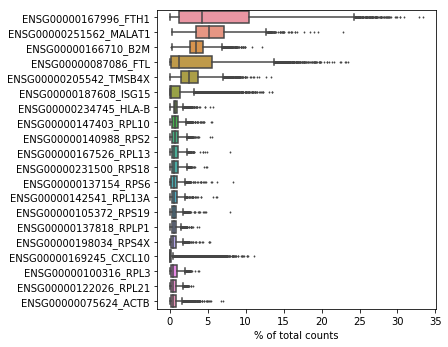
\includegraphics[scale=0.7]{hvg_top20}
%\caption{20 najzastupljenijih gena}
%\end{figure}

%\section{TF-IDF reprezentacija podataka}
%TODO
\section{Redukcija Dimenzionalnosti}
Bioinformatički podaci mogu imati veliki broj atributa(gena). U našem slučaju, postoje datoteke sa preko $30$ hiljada gena. Većina ovih gena su neinformativna, pri čemu je dosta njih ispunjeno nulama. Radi smanjenja vremena izvršavanja algoritama, pokušali smo da primenimo više različitih metoda redukcije dimenzionalnosti kao i metoda izbora atributa. U nastavku biće reči o izuzetno promenljivim genima(eng. Highly Variable Genes(HVG)), kao i o metodama nenegativne faktorizacije matrica(eng. Nonnegative Matrix Factorization(NMF) i PCA.

\subsection{Izuzetno promenljivi geni}
Prvi korak u smanjenju dimenzionalnosti podataka je izbor atributa(eng. feature selection). Izbor atributa pokušava da zadrži samo one atribute koji su \textit{informativni}, dok atributi, poput nula kolona ili atributi niske varijabilnosti se izbacuju. Metoda koja se pokazala kao kvalitetna za ovaj korak preprocesiranja podataka jeste metoda \textit{izuzetno promenljivih gena}(eng. Higly variable Genes(HVG)). U zavisnosti od skupa podataka, bira se prvih 1000 do prvih 5000 HVG-a \cite{luecken2019current}. Izbor HVG gena se vrši na sledeći način: za svaki gen se računa njegova prosečna ekspresija, a zatim se geni rasporede u korpe(eng. bins) na osnovu njihovih prosečnih ekspresija. Iz svake korpe se bira gen sa najvećim odnosom varijanse i prosečne vrednosti ekspresije. Upravo ti geni su HVG.

Prvenstveno, naše podatke smo log-transformisali, i zatim odredili HVG gene pomoću ScanPy biblioteke. Na primeru prve grupe podataka, dobili smo 1030 HVG-a.


\begin{figure}[h!]
\centering
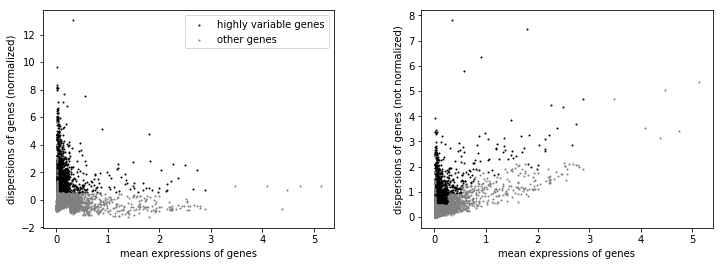
\includegraphics[scale=0.5]{hvg_izabrani}
\caption{Slike prikazuju odnos varijanse i prosečne ekspresije gena prve grupe podataka. Na slikama su crnom bojom obojene vrednosi HVG gena, a sivom vrednosti ostalih gena.}
\end{figure}

\subsection{Analiza glavnih komponenti}
Analiza glavnih komponenti(eng. Principal component Analysis) se pokazala kao kvalitetna metoda redukcije dimenzionalnosti i kao takva nalazi široke primene.

Na slici \ref{pca20} prikazan je procenat varijansi koje svaka od prvih 20 komponenti opisuje. Možemo primetiti da prva komponenta opisuje približno $25\%$ varijanse, a da nakon osme komponente, koločina varijanse koje ostale komponente opisuju je zanemarljiva. Da bi se opisalo $80\%$ varijansi skupa podataka, potrebno je čak $267$ komponenti. U ovom slučaju, sve komponente počev od deveta se mogu odbaciti, ali problem nastaju u tome što prvih osam komponenti opisuje svega $47\%$ varijanse. Zbog ovoga, u ovom radu nismo vršili detaljnije istraživanje nad PCA reprezentacijom podataka.


\begin{figure}[H]
\centering
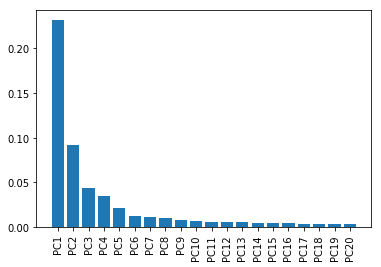
\includegraphics[scale=0.7]{pca20}
\caption{Procenat opisane varijansi prvih 20 komponenti dobijenih sa PCA}
\label{pca20}
\end{figure}



\subsection{Nenegativna faktorizacija matrice}
Nenegativna faktorizacija matrice(NMF) predstavlja metodu redukcije dimenzionalnosti koja automatski izvlači značajne atribute \cite{gillis2014and}. NMF nalazi primene u obradi teksta, obradi slika, a u ovom radu prikazaćemo rezultate primene nad bioinformatičkim podacima. Svojstvo koje matrica mora da zadovolji, kako bi nad njom bila primenjena NMF, jeste da je svaka vrednost te matrice nenegativna.

Neka je matrica $\mathbf{X} \in \mathbb{R}^{p\times n}$ koja čini skup podataka, pri čemu su kolone ove matrice instance, dok vrste atributi. Cilj NMF je dekompozicija matrice $\mathbf{X}$ na dve matrice $\mathbf{W} \in  \mathbb{R}^{p\times r} $ i $\mathbf{H} \in  \mathbb{R}^{r\times n}$ tako da važi $\mathbf{X} \approx \mathbf{W}\mathbf{H}$. Sve tri matrice su nenegativne.

\begin{figure}[H]
\centering
\caption{Slika preuzeta sa \cite{lamacraftausten}}
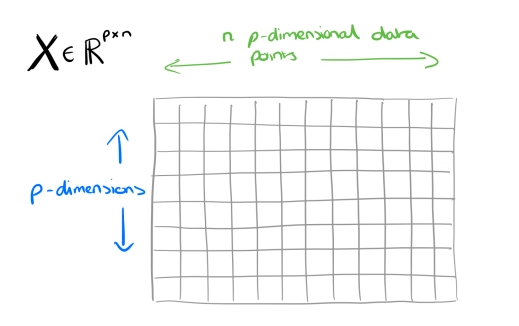
\includegraphics[scale=0.6]{x_nmf}
\end{figure}

Kolone matrice $\mathbf{W}$ možemo interpretirati kao bazne vektore, dok kolone matrice $\mathbf{W}$ predstavljaju koordinate instanci skupa podataka u toj novoj bazi.

\begin{figure}[H]
\centering

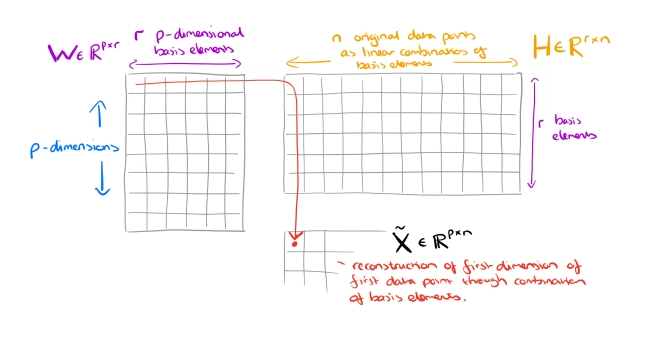
\includegraphics[scale=0.6]{wh_nmf}
\caption{Izvor slike \cite{lamacraftausten}}
\end{figure}


\subsubsection{NMF nad tekstualnim podacima}
\label{text_nmf}
Neka je data nenegativna matrica $\mathbf{X} \in \mathbb{R}^{p\times n}$ takva da svakoj koloni odgovara jedan dokument, dok vrste čine reči. Na poziciji $(i, j)$ te matrice nalazi se broj pojavljivanja i-te reči u j-tom dokumentu. Ovakve matrice nazivamo term-matricama. Primenom NMF nad  $\mathbf{X}$ dobijamo dve matrice  $(\mathbf{W}, \mathbf{H})$ tako da važi:


\begin{figure}[H]
\centering
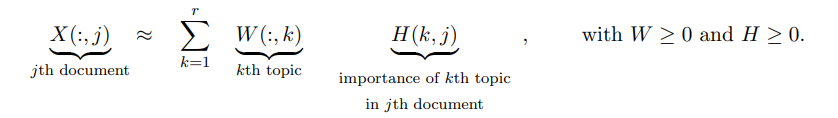
\includegraphics[width=\textwidth]{text_nmf}
\end{figure}


Kolone matrice $\mathbf{W}$ možemo interpretirati kao teme(eng. topics) dok vrednosti u matrici $\mathbf{H}$ čine težine koje govore koliko je neka tema bitna za neki dokument \cite{gillis2014and}.

\subsubsection{NMF nad prvom grupom podataka}
\label{genes_nmf}
U sekciji \ref{text_nmf} opisan je rezultat primene NMF nad tekstulanim podacima. Dakle, bazni vektori(kolone matrice $\mathbf{W}$) čine različite teme(sport, politika...) a težine u matrici $\mathbf{H}$ značajnost određenih tema za neki dokument. U slučaju naših podataka, kolone matrice $\mathbf{W}$ čine \textit{metagene}, dok vrenosti u $\mathbf{H}$ značajnost metagena za pojedinačne ćelije.\footnote{Uzeti u obzir da radimo sa transponovanim podacima, tj. vrste matrice $\mathbf{X}$ su instance(ćelije), a kolone geni. Zbog toga imamo novu reprezentaciju. $\mathbf{X}^T = \mathbf{H}^T\mathbf{W}^T$} Za broj metagena smo izabrali $50$, pa dobijamo novu reprezentaciju podataka dimenzija $15165 \times 50$. \footnote{Korišćena je implementacija NMF u okviru sklearn biblioteke \cite{scikit-learn}}


\section{Vizuelizacija}

U prethodnim sekcijama opisani su načini transformacija skupa podataka kako bi se dobila prikladna forma prihvatljiva od strane algoritama klasterovanja. U daljem radu biće korišćene dve verzije podataka \ref{plan}. \textbf{Prvu verziju} predstavljaju podaci dobijeni izborom zajedničkih gena za sve datoteke, zatim filtriranjem ćelija i gena metodama opisanim u \ref{elem_van_granica} i konačno prominemom NMF dekompozicije. \textbf{Drugu verziju} karakteriše još jedan korak, a to je izbor HVG gena pre primene NMF dekompozicije


\begin{figure}[h!]
\centering
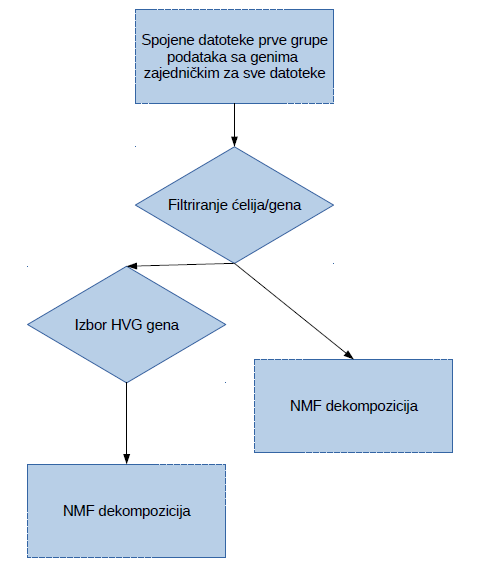
\includegraphics[scale=0.7]{plan}
\caption{Dijagram dobijanja dve verzije podataka}
\label{plan}
\end{figure}


Za vizuelizaciju podataka smo koristili t-SNE algoritam \cite{maaten2008visualizing}. Kao parametre algoritma, koristili smo:
\begin{itemize}
\item $perplexity =30$
\item $n\_iters = 5000$
\end{itemize}

a dobijeni rezultat za obe verzije prve grupe podataka predstavljen je na slici \ref{tsne_obe_verzije}. Možemo primetiti da je u drugoj verziji izdvojeno znatno više grupacija tačaka.

\begin{figure}[H]
	\centering
	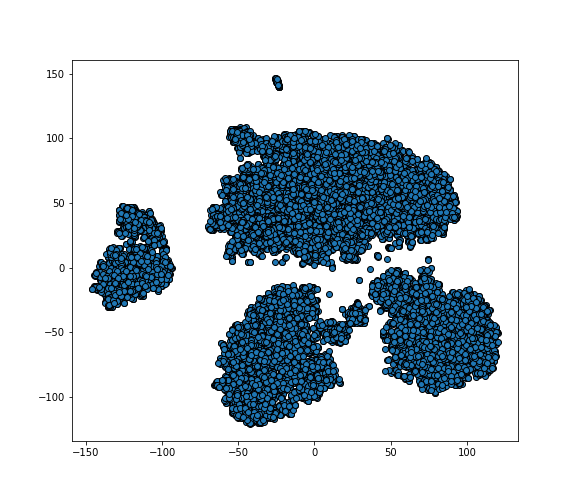
\includegraphics[scale=0.3]{tsne1}
	%\vspace{0.5in}
	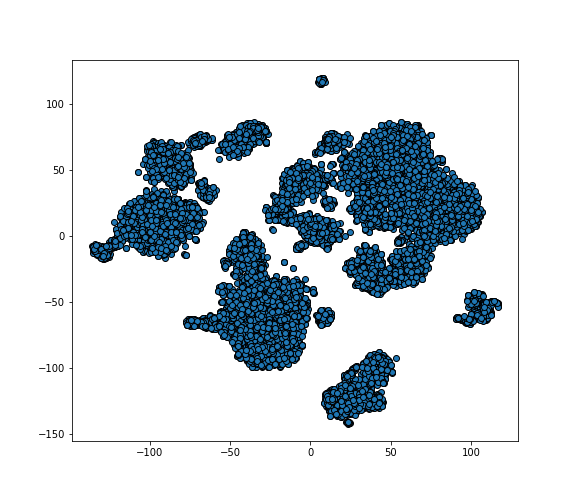
\includegraphics[scale=0.3]{hvg_tsne}
	\caption{Na slici (levo) prikazana je t-SNE projekcija prve vrezije prve grupe podataka, dok na slici imamo t-SNE projekciju druge verzije}
	\label{tsne_obe_verzije}
	%\vspace{1em}
\end{figure}





















\section{Klasterovanje prve grupe podataka}
Klasterovanje predstavlja tehniku koja je jako zastupljena u eksplorativnoj analizi podataka. U nastavku biće opisano nekoliko algoritama klasterovanja, kao i njihovi rezultati nad prvom grupom podataka.



\subsection{K-sredina}
K-sredina predstavlja jedan od najstarijih i najčešće korišćenih algoritama klasterovanja \cite{tan2016introduction}. Osnovni algoritam je jednostavan i iterativne prirode. U svakom koraku bira se $K$ nasumičnih centroida, svaka tačka skupa podataka se pridružuje najbližem centroidu, i na taj način se konstruišu klasteri. Zatim se na osnovu nekog kriterijuma ažuriraju centroidi i postupak se ponavlja sve dok  centroidi prestanu da se menjaju.

\begin{figure}[h!]
\centering
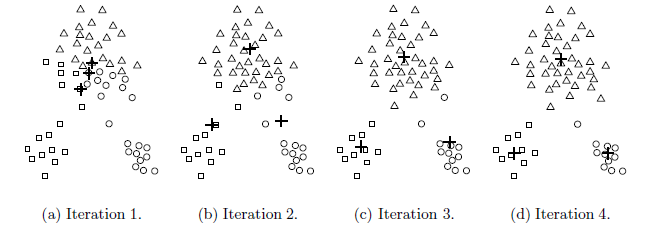
\includegraphics[scale=0.7]{kmeans_primer}
\caption{Primer izvršavanja algoritma k-sredina}
\label{kmeans_primer}
\end{figure}

Izbor centroida zavisi od izbora ciljnje funkcije. Standardna ciljnja funkcija za K-sredina je suma kvadrtanih grešaka(eng. Sum of squared errors(SSE)). SSE definišemo kao:

\begin{equation}
SSE = \sum_{i=1}^K\sum_{x_i \in C_i}dist(c_i, x)^2
\end{equation}

gde je \textit{dist} euklidsko rastojanje.

Na slikama \ref{kmeans_nmf_vise_klastera} i \ref{kmeans_grp1v2} vidimo rezultat algoritma k-sredina za različite vrednosti parametra k nad verzjiama, redom, jedan i dva. Konkretno, za pet klastera \ref{kmeans5_grp1v2}, možemo videti da k-sredina uspeva jasno da razdvoji klastere u slučaju druge verzije, mada prikazivanjem istih klastera nad prvom verzijom podataka, primećujemo da postoji dosta preklapanja. 

\begin{figure}[H]
	\centering
	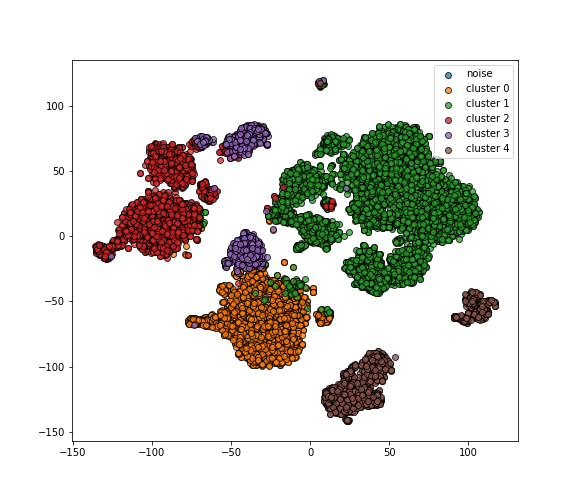
\includegraphics[scale=0.35]{kmeans5_grp1v2}
	%\vspace{0.5in}
	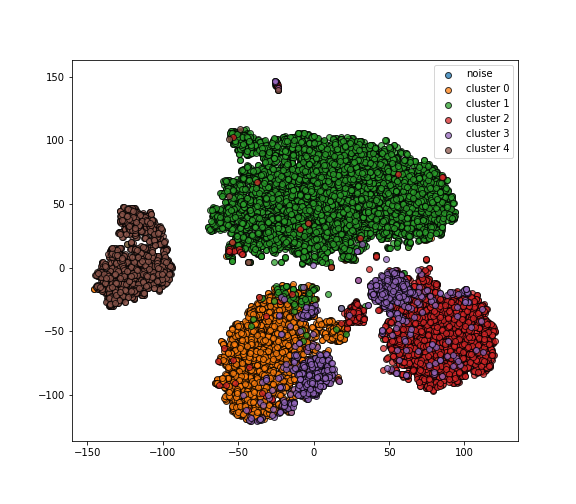
\includegraphics[scale=0.35]{kmeans5_grp1v2_nav1}
	\caption{Klasteri su dobijeni nad drugom verzijom podataka. Slika (levo) prikazuje vizuelizaciju klastera nad t-SNE projekcijom druge verzije, dok slika (desno) vizuelizaciju istih klastera ali nad t-SNE projekcijom prve verzije podataka. }
	\label{kmeans5_grp1v2}
	%\vspace{1em}
\end{figure}


\subsection{Spektralno klasterovanje}
Ako su podaci predstavljeni kao graf, gde su čvorovi instance, a grane povezuju bliske čvorove(zavisi od zadate mere bliskosti), tada jedan klaster čini komponenta povezanosti tog grafa. Spektralno klasterovanje je primer algoritma zasnovanog na grafovskoj reprezentaciji podataka.

\begin{figure}[h!]
\centering

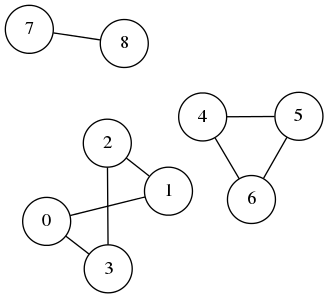
\includegraphics[scale=0.6]{komponente_povezanosti}
\caption{Graf sa tri komponente povezanosti}
\end{figure}

Neka je $\mathbf{G = (V, E)}$ \textit{neusmeren težinski graf} sa skupom čvorova $\mathbf{V} = \{v_1, v_2, ...., v_n\}$ i skupom grana $\mathbf{E}$. \textit{Matricu povezanosti} definišemo kao $\mathbf{W} = (w_{ij})$. Pretpostavimo da $w_{ij} \geq 0, \forall i, j$, tj sve težine su nenegativne. U slučaju da je $w_{ij} = 0$, čvorovi $i$ i $j$ nisu povezani.

Stepen čvora $v_i \in V$ definišemo kao \[deg(i) = \sum_{j=1}^{|V|} w_{ij}\].

Postoji više načina za računanje matrice povezanosti. U ovom radu koristili smo pristupu \textit{k-najbližih suseda}. Cilj ove metode je da poveže čvor $v_i$ sa $v_j$ ako je $v_j$ među prvih k najbližih suseda čvora $v_i$(važi i obrnuto). Ovom metodom dobijamo usmeren graf, pa jednostavnim eleminisanjem usmerenja grana dobijamo neusmerni graf povezanosti.

Glavna komponenta spektralnog klasterovanja je \textbf{graf Laplasijan} \cite{von2007tutorial}. \textit{Nenormalizovani graf Laplasijan} definisemo kao \[ L = D - W\] gde je D dijagonalna matrica takva da $d_{ii} = deg(i)$ (eng. degree matrix), a matrica $W$ matrica povezanosti.

Osnovni algoritam spektralnog klasterovanja je sledeći \cite{von2007tutorial}:

\SetKwInput{KwInput}{Input}         
\SetKwInput{KwOutput}{Output} 

\begin{minipage}{0.9\linewidth}%
\begin{algorithm}[H]
\SetAlgoLined
\KwInput{Skup podataka $D$, broj klastera $c$}
Izračunati matricu povezanosti metodom k-najbližih suseda\;
Izračunati Laplasijana $L$\;
Izračunati prvih $c$ sopstvenih vektora $s_1, s_2, ... s_c$\;
Izračunati prvih $c$ sopstvenih vektora $s_1, s_2, ... s_c$ matrice $L$. Neka je matrica $S \in \mathbb{R}^{n \times c}$ koja sadrži sopstvene vektore $s_1, s_2, ... s_c$ kao kolone. Tada je nova reprezentacija instance $a_i \in D, \forall i$ i-ta vrsta matrice $S$.\;
Izvršiti klasterovanje metodom k-sredina nad novom reprezentacijom podataka\;
 \KwOutput{Klasterovani podaci}
 \caption{Spektralno klasterovanje, osnovni algoritam}
\end{algorithm}
\end{minipage}

\verb||

\subsubsection{Spektralno klasterovanje nad prvom verzijom prve grupe podataka}
U okviru sekcije \ref{genes_nmf} prikazan je NMF oblik podataka prve grupe. Prvu grupu čini pet datoteka, tj datoteke GSM2560245, GSM2560246, GSM2560247, GSM2560248, GSM2560249. Koristili smo implementaciju spektralnog klasterovanja u okviru sklearn biblioteke. Lista bitnih parametara algoritma spektralno klasterovanja i njihove vrednosti su:
\begin{itemize}
\item $n\_cluster \in \{4, 5, 6, 7\}$
\item $affinity \in  \{nearest\ neighbors, precomputed\}$
\item $n\_neighbors \in \{10, 50, 124\}$
\item $metrika \in \{euklidsko\ rastojanje, kosinusno\ rastojanje, korelacija\}$
\end{itemize}

Prilikom konstruisanja matrice povezanosti, za broj suseda n\_neighbors korišćene su vrednosti iz skupa
$\{10, 50, 124\}$.\footnote{Vrednost 124 dobijena je zaokruživanjem vrednosti $\sqrt{broj\_instanci}$} Eksprimentisanjem sa različitim metrikama, ispostavlja se da za vrednost $n\_neighbors = 10$ dobijamo najbolje rezultate. Na slici \ref{spektralno_nmf_vise_klastera} možemo videti kako se spektralno klasterovanje ponaša za različit broj klastera. Deluje da se za $n\_cluster = 5$ dobijaju najbolji rezultati, pa u nastavku se fokusiramo na taj broj klastera\footnote{Kako spektralno klasterovanje koristi algoritam k-sredina, različita pokretanja algoritma mogu dati različite rezultate}. Kao mera kvaliteta korišćen je \textit{silueta koeficijent} i t-SNE algoritam za vizuelizaciju.

Na osnovu slika \ref{spektral_nmf_grp1_euklidsko}, \ref{spektral_nmf_grp1_cosine} i \ref{spektral_nmf_grp1_korelacija}, dobijaju se dosta slični rezultati za sve tri metrike. Jedino euklidsko rastojanje daje manji ukupni silueta koeficijent(\textbf{0.204863}) u odnosu na silueta koficijent dobijen kosinusnim rastojanjem(\textbf{0.444556}), odnosno silueta koficijent dobijen korišćenjem koeficijenta korelacije(\textbf{0.438462}) kao metrike rastojanja.

Slike \ref{spektral_nmf_grp1_cosine_bar} i \ref{raspodela_celija} prikazuju vezu između datoteka i klastera. Tako na primer, klaster 3 čine većinom ćelije iz datoteke GSM2560249 i nekolicina ćelija iz datoteke GSM2560248. Slično važi i za klaster 1, gde je većina ćelija iz jedne datoteke, tj iz GSM2560249. Uzeti u obzir da se skale grafikona razlikuju. Opis datoteka je prikazan u tabeli \ref{group1_metadata}.

\begin{figure}[H]
	\centering
	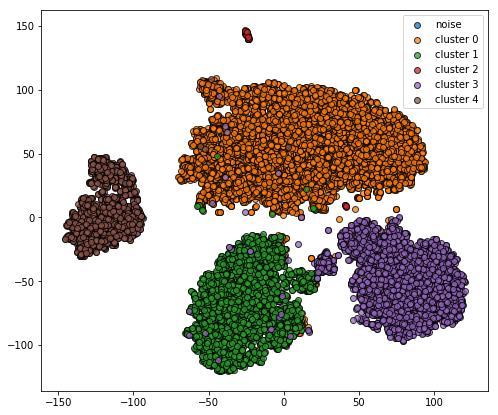
\includegraphics[scale=0.4]{spektral_nmf_grp1_cosine_bar}
	\caption{Spektralno klasterovanje sa kosinusnim rastojanjem}
	\label{spektral_nmf_grp1_cosine_bar}
	%\vspace{1em}
\end{figure}


\begin{figure}[H]
	

	\begin{subfigure}[normla]{0.3\textwidth}
		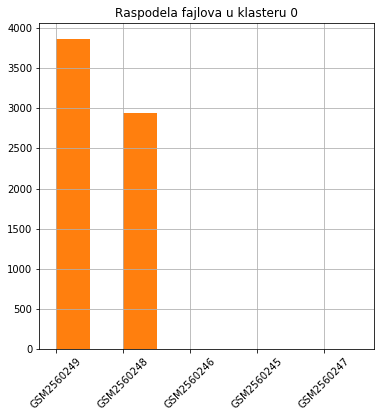
\includegraphics[scale=0.3]{bar_spektral_cosine_klaster0}
		\caption{Raspodela ćelija po datotekama koje čine klaster 0}
		\label{bar_spektral_cosine_klaster0}
	\end{subfigure}
	~
	\begin{subfigure}[normla]{0.3\textwidth}
		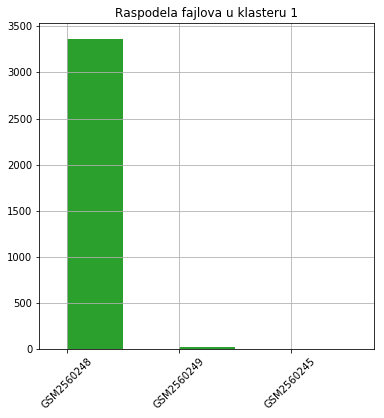
\includegraphics[scale=0.3]{bar_spektral_cosine_klaster1}
		\caption{Raspodela ćelija po datotekama koje čine klaster 1}
		\label{bar_spektral_cosine_klaster1}
	\end{subfigure}
	~
	\begin{subfigure}[normla]{0.3\textwidth}
		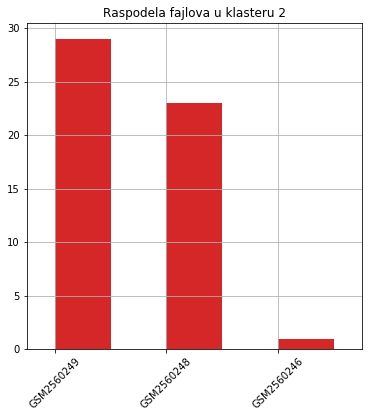
\includegraphics[scale=0.3]{bar_spektral_cosine_klaster2}
		\caption{Raspodela ćelija po datotekama koje čine klaster 2}
		\label{bar_spektral_cosine_klaster2}
	\end{subfigure}
	~
	\begin{subfigure}[normla]{0.3\textwidth}
		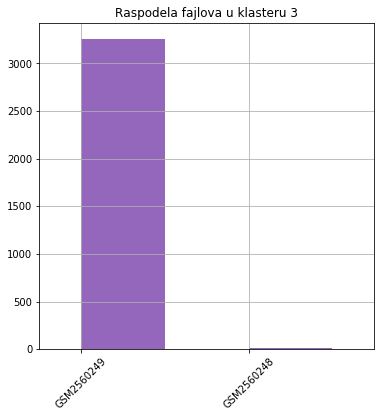
\includegraphics[scale=0.3]{bar_spektral_cosine_klaster3}
		\caption{Raspodela ćelija po datotekama koje čine klaster 3}
		\label{bar_spektral_cosine_klaster3}
	\end{subfigure}
	~
	\begin{subfigure}[normla]{0.3\textwidth}
		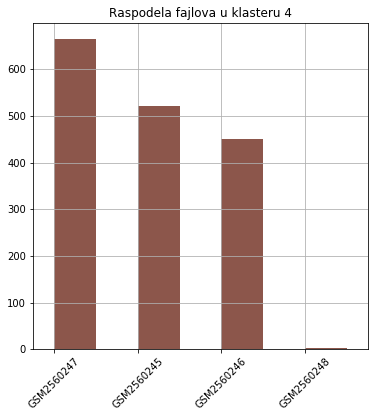
\includegraphics[scale=0.3]{bar_spektral_cosine_klaster4}
		\caption{Raspodela ćelija po datotekama koje čine klaster 4}
		\label{bar_spektral_cosine_klaster4}
	\end{subfigure}	
	\caption{Raspodela ćelija po datotekama za svaki klaster}
	
\label{raspodela_celija}
\end{figure}



\subsubsection{Spektralno klasterovanje nad drugom verzijom prve grupe podataka}

U prethodnoj sekciji videli smo da spektralno klasterovanje, u kombinaciji sa NMF dekompozicijom uspeva da pronađe jasno razdvojene(na osnovu t-SNE prikaza) klastere. Trend se nastavlja i na primeru druge verzije podataka \ref{hvg_nmf_spectral}. Na slici \ref{spektral_v2_prikaz_na_v1} možemo videti šta se dešava ako dobijene labele klastera vizuelizujemo i nad t-SNE projekcijom za prvu verziju podataka. Interesantno je da su dosta klastera skoro pa identična.

\begin{figure}[ht]
	\centering
	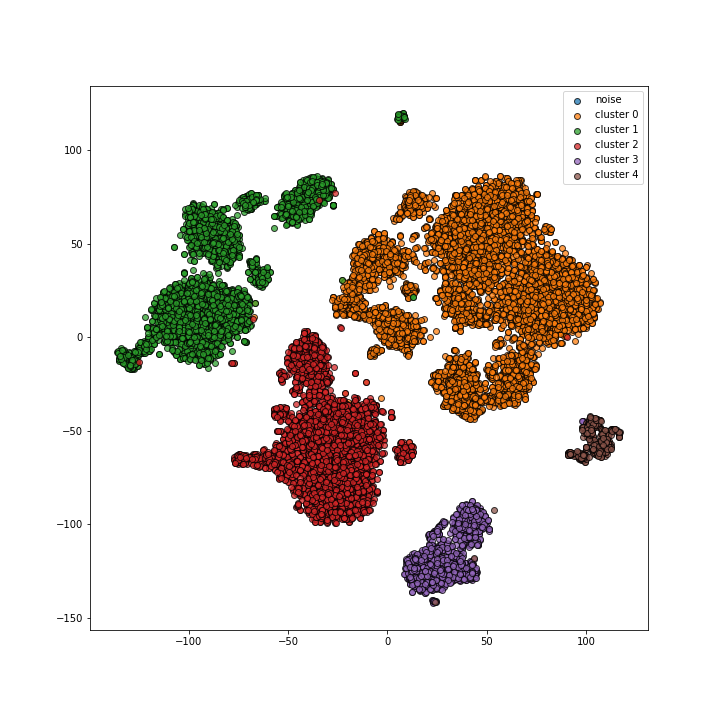
\includegraphics[scale=0.25]{spektral_v2_5}
	%\vspace{0.5in}
	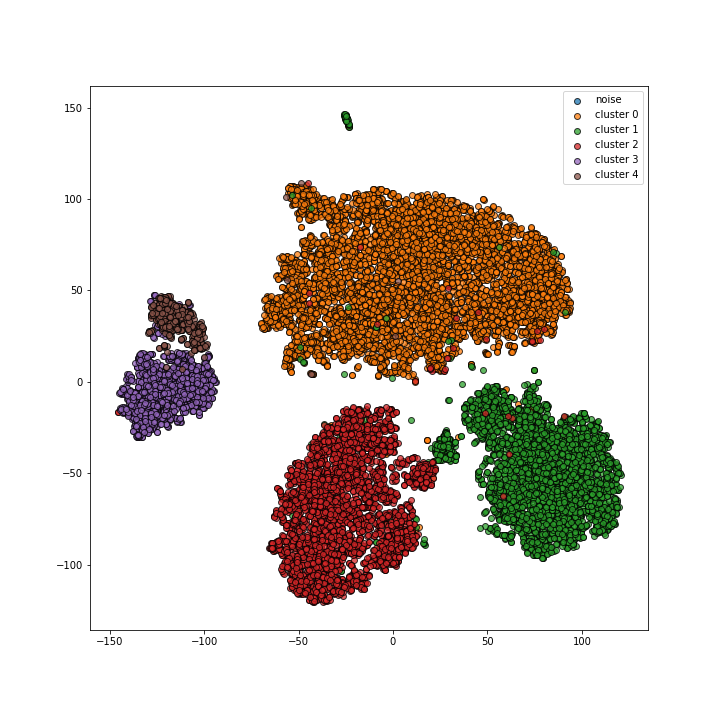
\includegraphics[scale=0.25]{spektral_v2_prikaz_na_v1}
	\caption{Spektralno klasterovanje dobijeno nad drugom verzijom podataka, prikaz nad t-SNE projekcijom druge verzije (levo) i prikaz nad t-SNE projekcijom prve verzije (desno).}
	\label{spektral_v2_prikaz_na_v1}
	%\vspace{1em}
\end{figure}



\subsection{Hijerarhijsko klasterovanje}

Hijerahijsko klasterovanje predstavlja još jednu metodu klasterovanja čija je osnovna karakteristika, kao što i sam naziv govori, konstruisanje \textit{hijerarhija}. Postoje dve vrste hijerarhijskog klasterovanja, i to:
\begin{itemize}
\item sakupljajući(eng. agglomerative)
\item razdvajajući(eng. divisive)
\end{itemize}

Osnovna razlika ove dve vrste je to što, u sakupljajućem slučaju, svaka instanca predstavlja odvojen klaster. Iterativno se zatim,na osnovu neke mere bliskosti, spajaju najbliži klasteri sve dok ne ostane samo jedan klaster. U slučaju razdvajajućeg hijerarhijskog algoritma, proces je analogan, pri čemu se počinje od jednog klastera, a zatim se instance iterativno razdvajaju.
U nastavku biće više reči o sakupljajućem hijerarhijskom algoritmu, kao i njegovim varijacima. Opšti algoritam je oblika:

\begin{minipage}{1\linewidth}%
\begin{algorithm}[H]
\SetAlgoLined
\KwInput{skup podataka $D$ ili matrica bliskosti $P$}
Ako je prosleđen skup podataka, izračunati matricu bliskoti $P$\;
 \Repeat{dok nije ostao samo jedan klaster}{
	Spoji dva $"$najbliža$"$ klastera\;
	Transformiši matricu bliskoti $P$\;
 }
 \KwOutput{Klasterovani podaci}
 \caption{Osnovni sakupljajući hijerarhijski algoritam}
\end{algorithm}
\end{minipage}

\verb||

Definicija mere bliskosti je ono što razlikuje različitie vrste sakupljajućeg hijerarhijskog algoritma \cite{tan2016introduction}. Standardne mere bliskosti su:
\begin{itemize}
\item Single veza
\item Complete veza
\item Average veza
\item Ward-ova veza
\end{itemize}

Upoređene su sve četiri mere bliskosti nad prvom grupom podataka, pri čemu su najbolji rezultati postignuti sa Ward-ovom merom. Na slici \ref{dendogram} prikazan je dendogram dobijen korišćenjem biblioteke SciPy \cite{2020SciPy-NMeth}, dok na slici \ref{ward_clustering} prikazan je rezultat dobijen funkcijom AgglomerativeClustering u okviru scikit-learn biblioteke i to sa parametrima:
\begin{itemize}
\item $n\_clusters = 5$
\item $linkage = "ward"$
\end{itemize}


\begin{figure}[H]
	\centering
	\begin{subfigure}[normla]{0.4\textwidth}
		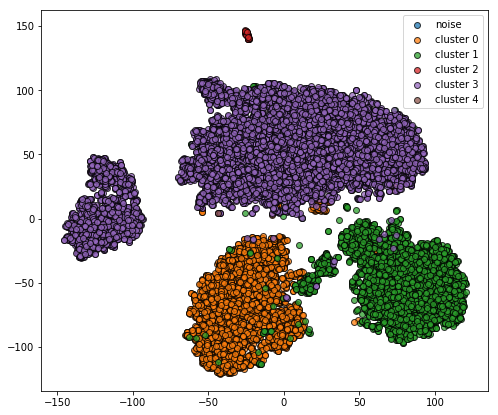
\includegraphics[scale=0.3]{ward_clustering}
		\caption{Hijerarhijsko klasterovanje sa Ward-ovom merom za 5 klastera}
		\label{ward_clustering}
	\end{subfigure}
	~
	\begin{subfigure}[normla]{0.4\textwidth}
		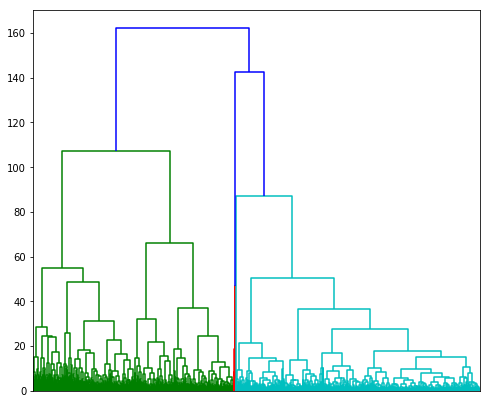
\includegraphics[scale=0.3]{dendogram}
		\caption{Dendogram Ward-ovog hijerarhijskog algoritma}
		\label{dendogram}
	\end{subfigure}
		\caption{Na slici (a) prikazani su dobijeni klasteri hijerarhijskim algoritmom sa Ward-ovom merom, dok na slici (b) ceo dendogram hijerarhijskog algoritma, takođe sa Ward-ovom merom. Uzeti u obzir da su slike nezavisne jedna od druge.}
\label{spektral_nmf_grp1_cosine}
\end{figure}


Za drugu verziju podataka, Ward-ova mera daje dosta slične, pa gotovo iste rezultate kao i algoritam k-sredina \ref{ward_nav2}. Takođe, preklapanja koja su se javljala u slučaju k-sredina algoritma, javljaju se i ovde \ref{wardv2_nav1}, pa se nameće pitanje, koja je od ove dve verzije podataka reprezentativnija.

\begin{figure}[H]
\centering
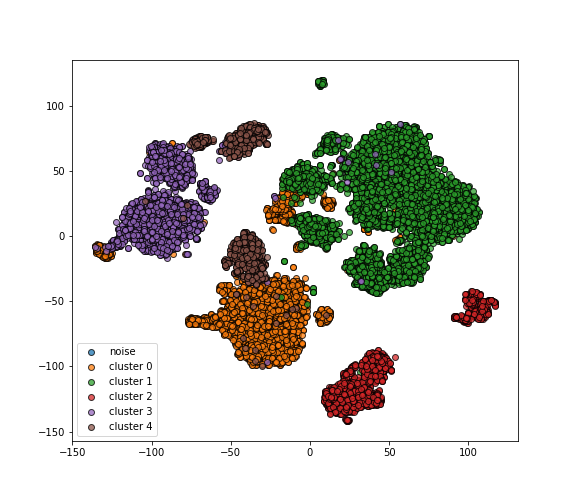
\includegraphics[scale=0.5]{ward_nav2}
\caption{Klasteri dobijeni Ward-ovim hijerarhijskim klasterovanjem nad verzijom dva}
\label{ward_nav2}
\end{figure}

\begin{figure}[H]
\centering
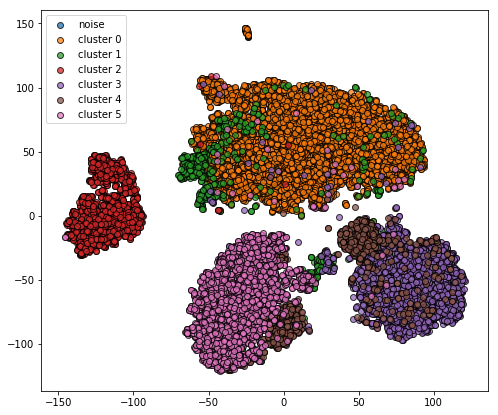
\includegraphics[scale=0.5]{wardv2_nav1}
\caption{Klasteri dobijeni Ward-ovim hijerarhijskim klasterovanjem nad verzijom dva, prikazani nad verzijom jedan.}
\label{wardv2_nav1}
\end{figure}









\subsection{Klasterovanje zasnovano na gustini}

Algoritmi zasnovani na gustini lociraju $"$guste$"$ regione prostora razdvojene regionima manje gustine \cite{tan2016introduction}. Osnovna karakteristika ovih algoritama je to što mogu da prepoznaju klastere proizvoljnog oblika. Najpoznatiji algoritam koji se zasniva na ovom principu je DBSCAN \cite{Ester96adensity-based}.

\subsubsection{DBSCAN}
\label{DBSCAN}

DBSCAN se pokazao kao izuzetno dobar algoritam za pronalaženje klastera različitih oblika. Algoritam se sastoji od dva parametra, \textit{minPts} i \textit{eps}. Takođe, autori DBSCAN-a su predložili metodu \textit{k-dist plot}-a kako bi se broj parametara algoritma sveo na svega jedan. Drugim rečima za dati minPts, pomoću k-dist plot-a, moguće je automatski odrediti prikladno \textit{eps}. Osnovna karakteristika DBSCAN-a je podela tačaka(instanci) na 3 vrste, i to na tačke jezgra, granične tačke i šum \ref{core_pts}. 

Da bismo definisali tačke jezgra, uvodimo pojam \textit{eps-okruženje}.
Eps-okruženje tačke p predstavlja skup tačaka $N_{eps}(p)$ definisan kao 

\begin{equation}
	N_{eps}(p) = \{ q\ |\ dist(p, q) \leq eps \}
\end{equation}


\begin{figure}[h!]
\centering
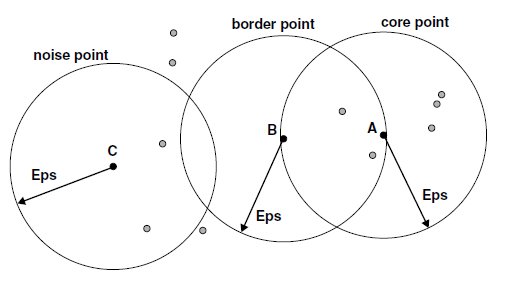
\includegraphics[scale=0.7]{core_pts}
\caption{Šum, granične tačke i tačke jezgra}
\label{core_pts}
\end{figure}

Ako je za tačku p poznata njeno eps-okruženje i ako važi da 
\begin{equation}
	N_{eps}(p) \geq minPts
\end{equation}

tada kažemo da je tačka p \textit{tačka jezgra}. Za tačku q koja nije tačka jezgra ali važi da u njenom eps-okruženju pripada neka tačka jezgra, onda za q kažemo da je \textit{granična tačka}. I na kraju, ako tačka x nije ni tačka jezgra, ni granična, onda nju smatramo kao \textit{šum}.
Kada se odrede tipovi tačaka, susedne tačke jezgra\footnote{Tačke p i q su susedne ako važi da $p \in N_{eps}(q)$ ili $q \in N_{eps}(p)$ } se spajaju u jedan klaster, a granične tačke se pridružuju njima najbližim klasterima.

\subsubsection{Određivanje parametara eps i minPts}
U sekciji \ref{DBSCAN} je spomenuto da DBSCAN čine dva parametra, i to \textit{minPts} i \textit{eps}. Zajedno, ova dva parametra određuju koliko \textit{retke} klastere očekujemo. Tako za manje vrednosti \textit{eps} i veće vrednosti \textit{minPts}, dobijamo guste klastere, dok za veće vrednosti \textit{eps} i manje vrednosti \textit{minPts} dobijamo \textit{retke} klastere. Odabir parametara ima ključnu ulogu na performanse DBSCAN-a. Takođe često se ne zna $"$gustina$"$ klastera, što znatno otežava problem. Zbog ovoga, autori DBSCAN-a su predložili heuristiku k-dist plot\footnote{Vrednost k u nazivu k-dist je jednaka minPts.} za određivanje prikladnog eps-a na osnovu zadate vrednosti za minPts. Procedura je sledeća, za svaku tačku se nalazi njen \textit{minPts-najbliži sused}. Zatim se dobijeni niz minPts-najbližih suseda sortira, i traži se vrednost u kojoj dobijena $"$kriva$"$ naglo menja pravac. Na slici \ref{kdist_plot} prikazan je k-dist plot za prvu verziju prve grupe podataka za $minPts = 10$.

\subsubsection{DBSCAN nad prvom grupom podataka}

Na osnovu slike \ref{kdist_plot}, odabrali smo da vredonosti \textit{eps} budu iz intervala $[3, 8]$. Interval $[3, 8]$ smo ekvidistantno podelili na 5 delova i dobijene vrednosti smo koristili za vrednost eps-a, dok je vrednost minPts postavljena na 10. Sa ovim parametrima, primenili smo DBSCAN nad NMF reprezentacijom prve grupe podata. Ipak, DBSCAN nije uspeo da detektuje klastere, čak nije prepoznao šumove, pa je sve tačke stavio u jedan klaster. Slični rezultati se dobijaju ako DBSCAN primenimo nad formatu prve grupe opisanom u \ref{elem_van_granica}. 

Takođe, primenili smo i algoritam OPTICS \cite{ankerst1999optics}, ali rezultati su takođe bili nezadovoljavajući, pa neće biti detaljnije diskusije o navedenom algoritmu.

Na osnovu slike \ref{kdist_plot} može se zaključiti da su sve tačke relativno $"$blizu$"$ jedna drugoj. To možemo takođe videti iz vrednosti silueta koeficijnata dobijenih spektralnim klasterovanjem. Naime, kada je silueta koficijent blizak nuli, to ukazuje na preklapanje klastera. To možemo videti i u slučaju spektralnog klasterovanja, konkretno za spektralno klasterovanje i euklidsko rastojanje \ref{spektral_nmf_grp1_euklidsko_A}. Interesantno je da je ipak, na osnovu vizuelizacije t-SNE-om, spektralno klasterovanje uspelo da razdvoji klastere.


\begin{figure}[h!]
\centering
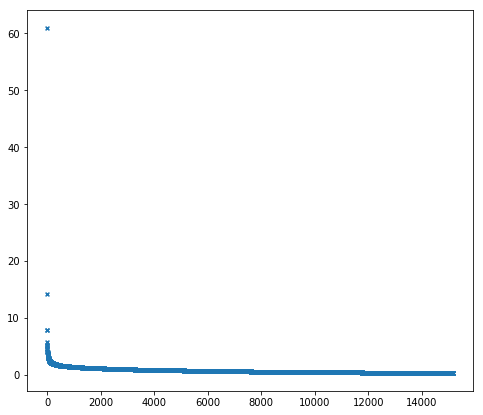
\includegraphics[scale=0.45]{kdist_plot}
\caption{K-dist plot za NMF reprezentaciju prve grupe podataka, za $minPts=10$}
\label{kdist_plot}
\end{figure}

Slične rezultate dobijamo i sa drugom verzijom podataka, pri čemu u ovom slučaju nekolicina tačaka je označena kao šumovi, dok većina pripada jednom klasteru. Za parametre smo koristili 
\begin{itemize}
\item $eps = 0.3$
\item $minPts = 50$
\end{itemize}
a vizuelni prikaz je predstavljen na slici \ref{dbscan_v2}.

Ovim dolazimo do zaključka da algoritmi zasnovani na gustini nisu primenljivi nad ovakvom vrstom podataka.


\begin{figure}[ht]
	\centering
	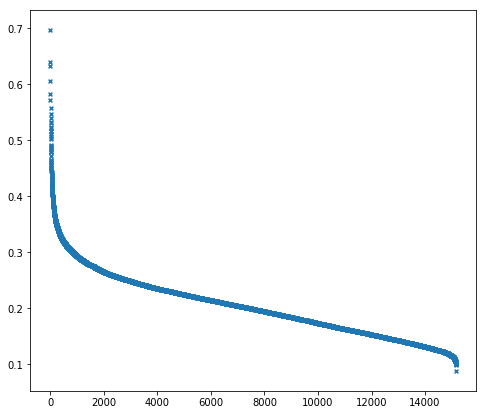
\includegraphics[scale=0.3]{kdist_v2}
	%\vspace{0.5in}
	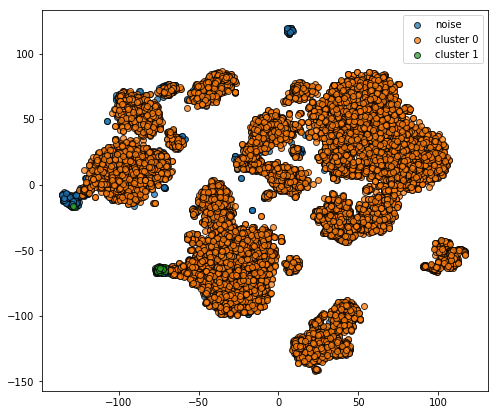
\includegraphics[scale=0.3]{dbscan_v2}
	\caption{Na slici (levo) vidimo k-dist plot za drugu verziju prve grupe podataka, dok slika (desno) prikazuje t-SNE vizuelizaciju dobijenih klastera DBSCAN algoritmom}
	\label{dbscan_v2}
	%\vspace{1em}
\end{figure}














\section{Zaključak}
U ovom radu primenili smo više algoritama za klasterovanje nad PBMC ćelijama. Zbog prirode podataka, velika pažnja je posvećena redukciji dimenzionalnosti. Koristili smo dve verzije reprezentacije podataka, pri čemu dobijamo dobre rezultate za obe verzije. Algoritam spektralnog klasterovanja se pokazao kao kvalitetan pristup ovom problemu, dok sa algoritmima zasnovanim na gustini nismo imali dosta uspeha. Za dalji rad planiramo upotrebu još nekoliko metoda za preprocesiranje podataka, poput tf-idf-a, kao i primeniti druge pristupe za redukciju dimenzionalnosti, poput autoenkodera.





















\appendix
\section{Opisi datoteka koje čine skup podataka}
\begin{center}
\begin{table}[H]
\caption{Metapodaci za prvu grupu}
\begin{adjustbox}{width=1\textwidth}
\begin{tabularx}{\textwidth}{llY}
\toprule
     SAMPLE & GENOME &                                                                                                                                                                                                                  DESCRIPTION \\
\midrule
 GSM2560245 &   hg19 &                                                              batch 1 sample A; single cell RNA-seq\_SLE patients (well 1); Homo sapiens; subject status: SLE patient; cell type: peripheral blood mononuclear cells (PBMCs);  \\
 GSM2560246 &   hg19 &                                                              batch 1 sample B; single cell RNA-seq\_SLE patients (well 2); Homo sapiens; subject status: SLE patient; cell type: peripheral blood mononuclear cells (PBMCs);  \\
 GSM2560247 &   hg19 &                                                              batch 1 sample C; single cell RNA-seq\_SLE patients (well 3); Homo sapiens; subject status: SLE patient; cell type: peripheral blood mononuclear cells (PBMCs);  \\
 GSM2560248 &   hg19 &                       batch 2 control; single cell RNA-seq\_SLE patients (6 hours control); Homo sapiens; subject status: SLE patient; cell type: peripheral blood mononuclear cells (PBMCs); stimulated with: none (control) \\
 GSM2560249 &   hg19 &  batch 2 stim (IFN-beta); single cell RNA-seq\_SLE patients (6 hours IFN-b stimulation); Homo sapiens; subject status: SLE patient; cell type: peripheral blood mononuclear cells (PBMCs); stimulated with: IFN-beta for 6hrs \\
\bottomrule
\end{tabularx}
\end{adjustbox}
\label{group1_metadata}
\end{table}
\end{center}



\begin{center}
\begin{table}[H]
\caption{Metapodaci za drugu grupu}
\begin{adjustbox}{width=1\textwidth}
\begin{tabularx}{\textwidth}{llY}
\toprule
     SAMPLE &             GENOME &                                                                                                                                                                                  DESCRIPTION \\
\midrule
 GSM3087619 &             GRCh38 &                                                                            DTM-X\_PBMC\_live; whole blood; Homo sapiens; isolation: Ficoll; fixation: Live; resuspension: PBS; cell type: PBMC \\
 GSM3478792 &             GRCh38 &                                                                                                                    Patient1\_Nonmalignant; PBMC; Homo sapiens; condition: Normal PBMC T Cells \\
 GSM3892571 &             GRCh38 &                                     PBMC\_HV; PBMC from a sex- and age-matched healthy volunteer (HV); Homo sapiens; disease diagnosis: Healthy; tissue: PBMC; manipulation: Freshly isolated \\
 GSM3169075 &  GRCh38 version 90 &  Healthy human PBMCs; PBMC\_scRNA-seq; Homo sapiens; subject status: healthy donor; cell type: Peripheral blood mononuclear cells (PBMCs); barcode coordinate: tag CB; umi coordinate: tag UB \\
 GSM3374613 &               hg38 &                                                                                                                  lna\_cell\_pbmc\_original; Human PBMCs; Homo sapiens; sample type: Human PBMCs \\
 GSM3374614 &               hg38 &                                                                                                                 lna\_cell\_pbmc\_resampled; Human PBMCs; Homo sapiens; sample type: Human PBMCs \\
\bottomrule
\end{tabularx}
\end{adjustbox}
\label{group2_metadata}
\end{table}
\end{center}



\section{Dodatne vizuelizacije klastera}



\begin{figure}[H]
\centering
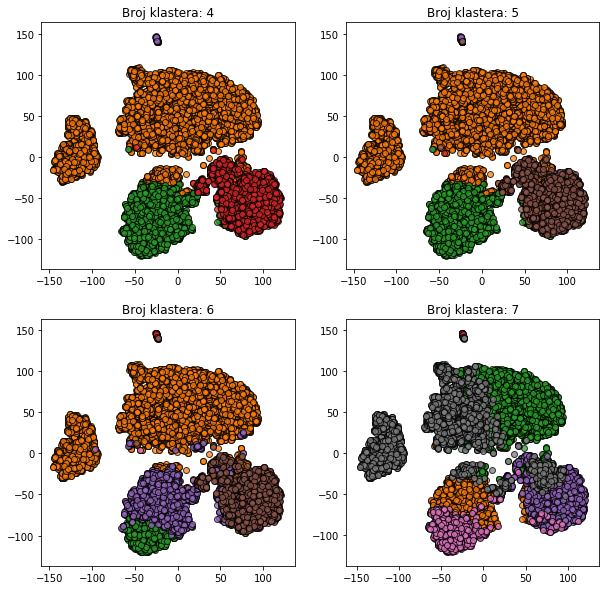
\includegraphics[scale=0.6]{kmeans_nmf_vise_klastera}
\caption{K-sredina nad prvom verzijom prve grupe podataka}
\label{kmeans_nmf_vise_klastera}
\end{figure}



\begin{figure}[H]
\centering
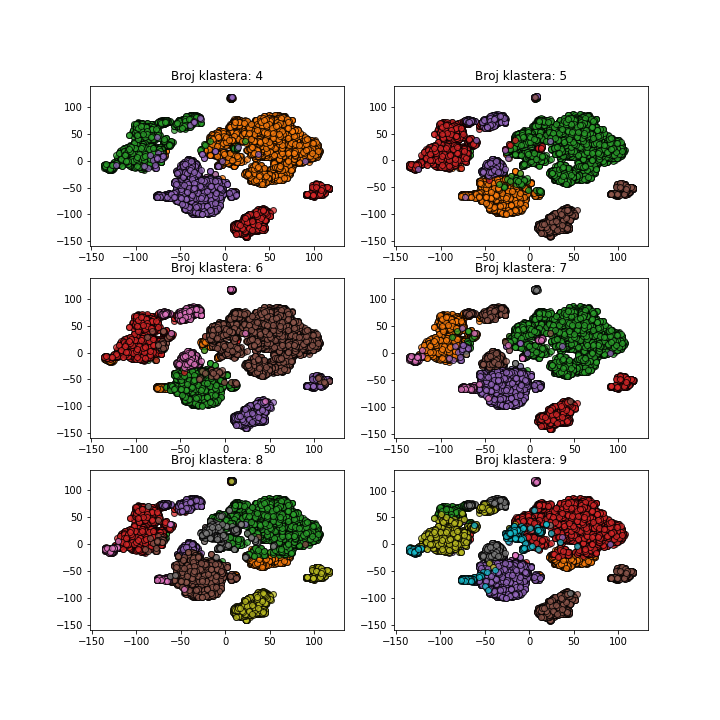
\includegraphics[scale=0.6]{kmeans_grp1v2}
\caption{K-sredina nad drugom verzijom druge grupe podataka}
\label{kmeans_grp1v2}
\end{figure}



\begin{figure}[H]
\centering
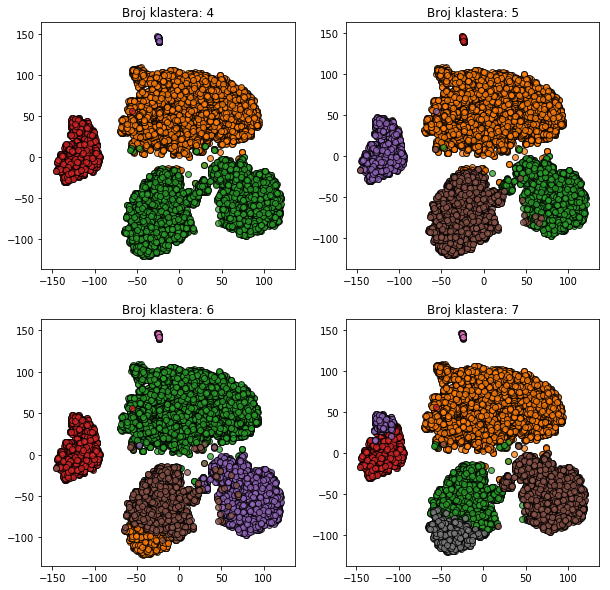
\includegraphics[scale=0.6]{spektralno_nmf_vise_klastera}
\caption{Spektralno klasterovanja nad prvom verzijom prve grupe podataka za različite vrednosti broja klastera}
\label{spektralno_nmf_vise_klastera}

\end{figure}

\begin{figure}[H]
	\centering
	
	\begin{subfigure}[normla]{0.5\textwidth}
		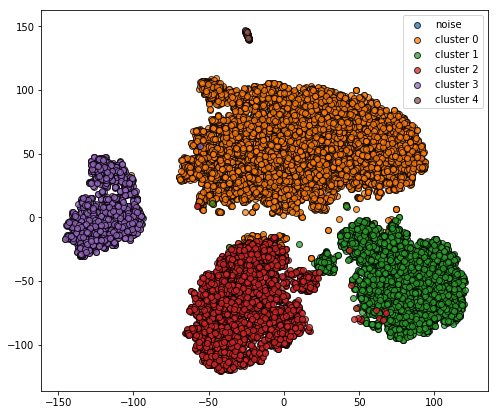
\includegraphics[scale=0.3]{spektral_nmf_grp1_euklidsko}
		\caption{Vizuelni prikaz klastera}
		\label{spektral_nmf_grp1_euklidsko_A}
	\end{subfigure}
	~
	\begin{subfigure}[normla]{0.4\textwidth}
		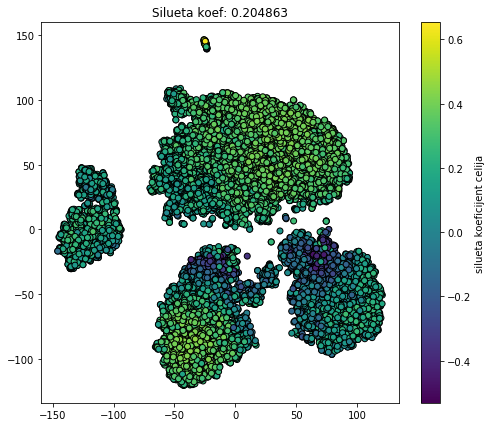
\includegraphics[scale=0.3]{spektral_nmf_grp1_euklidsko_silueta}
		\caption{Vizuelni prikaz silueta vrednosti pojedinačnih tačaka}
		\label{spektral_nmf_grp1_euklidsko_B}
	\end{subfigure}
	\caption{Spektralno klasterovanje sa \textit{euklidskim} rastojanjem. Na slici (a) klasteri su prikazani različitim bojama, dok na slici (b) boja jedne tačke zavisi od njenog silueta koeficijenta. Svetlije boje ukazuju na veću vrednost silueta koeficijenta, dok tamnije manju. Ukupan silueta koeficijent je \textbf{0.204863}}
\label{spektral_nmf_grp1_euklidsko}
\end{figure}


\begin{figure}[H]
	\centering

	\begin{subfigure}[normla]{0.5\textwidth}
		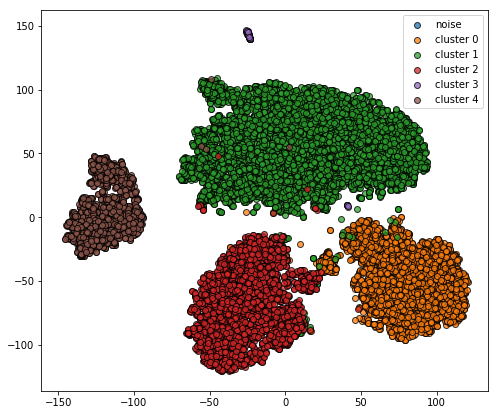
\includegraphics[scale=0.3]{spektral_nmf_grp1_cosine}
		\caption{Vizuelni prikaz klastera}
		\label{spektral_nmf_grp1_cosine_A}
	\end{subfigure}
	~
	\begin{subfigure}[normla]{0.4\textwidth}
		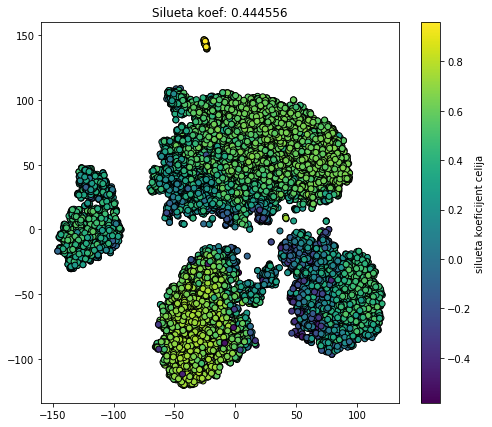
\includegraphics[scale=0.3]{spektral_nmf_grp1_cosine_silueta}
		\caption{Vizuelni prikaz silueta vrednosti pojedinačnih tačaka}
		\label{spektral_nmf_grp1_cosine_B}
	\end{subfigure}
		\caption{Spektralno klasterovanje sa \textit{kosinusnim} rastojanjem. Na slici (a) klasteri su prikazani različitim bojama, dok na slici (b) boja jedne tačke zavisi od njenog silueta koeficijenta. Svetlije boje ukazuju na veću vrednost silueta koeficijenta, dok tamnije manju. Ukupan silueta koeficijent je \textbf{0.444556}}
\label{spektral_nmf_grp1_cosine}
\end{figure}


\begin{figure}[H]
	\centering
	
	\begin{subfigure}[normla]{0.5\textwidth}
		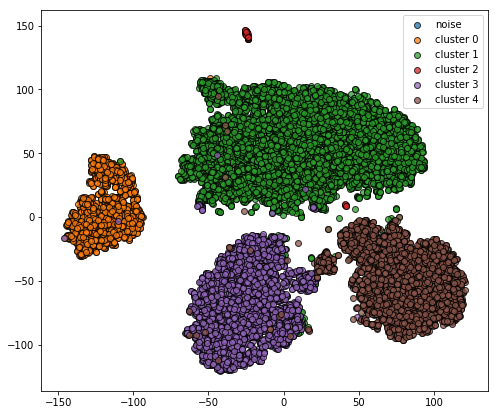
\includegraphics[scale=0.3]{spektral_nmf_grp1_korelacija}
		
		\caption{Vizuelni prikaz klastera}
		\label{spektral_nmf_grp1_korelacija_A}

	\end{subfigure}
	~
	\begin{subfigure}[normla]{0.4\textwidth}
		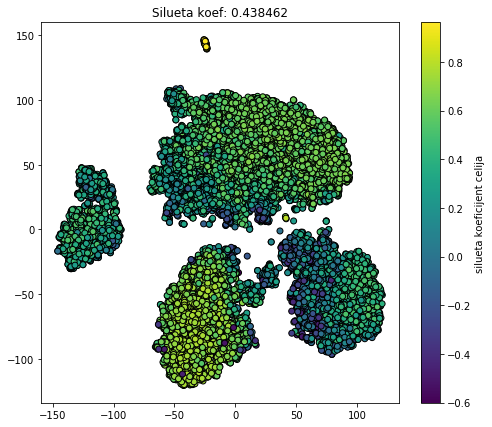
\includegraphics[scale=0.3]{spektral_nmf_grp1_korelacija_silueta}
		\caption{Vizuelni prikaz silueta vrednosti pojedinačnih tačaka}
		\label{spektral_nmf_grp1_korelacija_B}
	\end{subfigure}
	\caption{Spektralno klasterovanje sa \textit{koeficijentom korelacije} kao mera rastojanja. Na slici (a) klasteri su prikazani različitim bojama, dok na slici (b) boja jedne tačke zavisi od njenog silueta koeficijenta. Svetlije boje ukazuju na veću vrednost silueta koeficijenta, dok tamnije manju. Ukupan silueta koeficijent je \textbf{0.438462}}
\label{spektral_nmf_grp1_korelacija}
\end{figure}

\begin{figure}[h!]
\centering
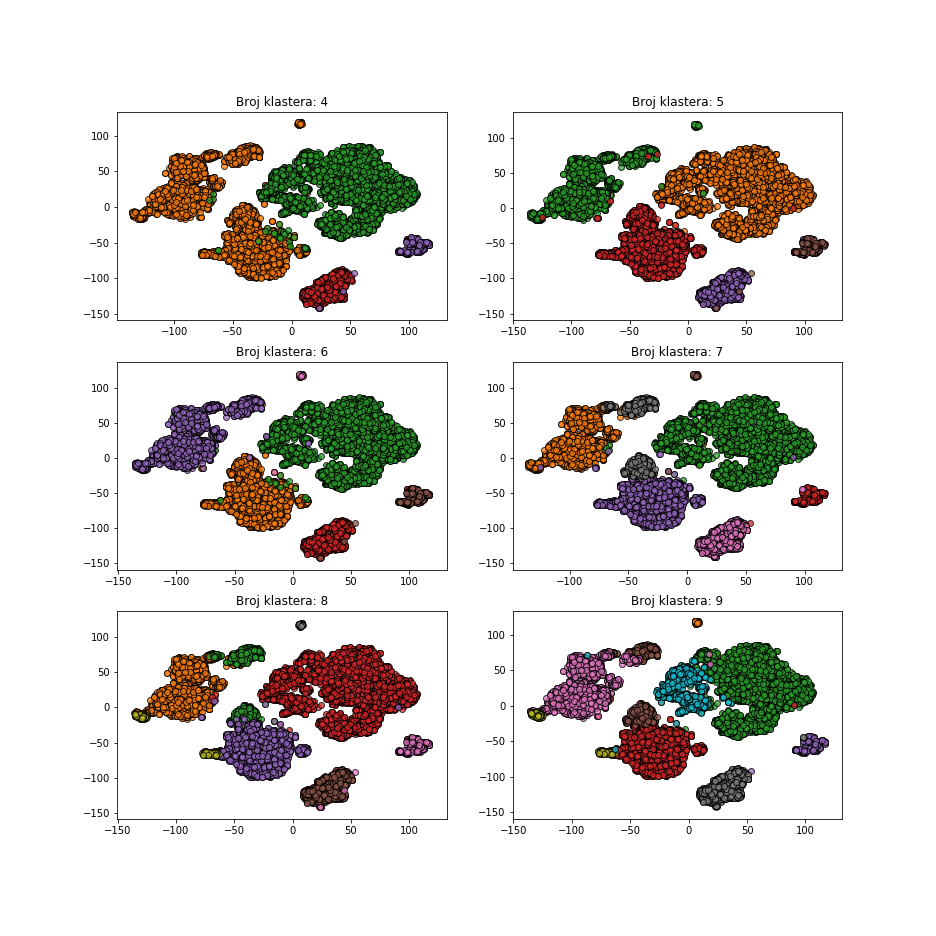
\includegraphics[scale=0.4]{hvg_nmf_spectral}
\caption{Spektralno klasterovanja nad drugom verzijom prve grupe podataka za različit broj klastera}
\label{hvg_nmf_spectral}
\end{figure}

\newpage
\bibliographystyle{plain}
\bibliography{citati.bib}

\end{document}